\section{Theoretical background and literature review}
\label{section:2}

\subsection{Rarefied flow}
The expression rarefied flow refers to a set of flow conditions where the gas is so rarefied that the continuum assumption of ordinary fluid mechanics ceases to be valid \cite{aerothermonotes}. Because of this, statistical mechanics has to be employed to describe it, rather than continuum mechanics.

It is possible to determine whether a flow is rarefied through the Knudsen number, a dimensionless number defined as in \autoref{eq:knudsen}, where $\lambda$ is the mean free path of the flow molecules and $l$ is a characteristic length of the flow.
\begin{equation}
    Kn=\frac{\lambda}{l}
    \label{eq:knudsen}
\end{equation}
As it is possible to see from \autoref{fig:regimes}, flows can be divided into three categories based on Knudsen number:
\begin{figure}[ht]
    \centering
    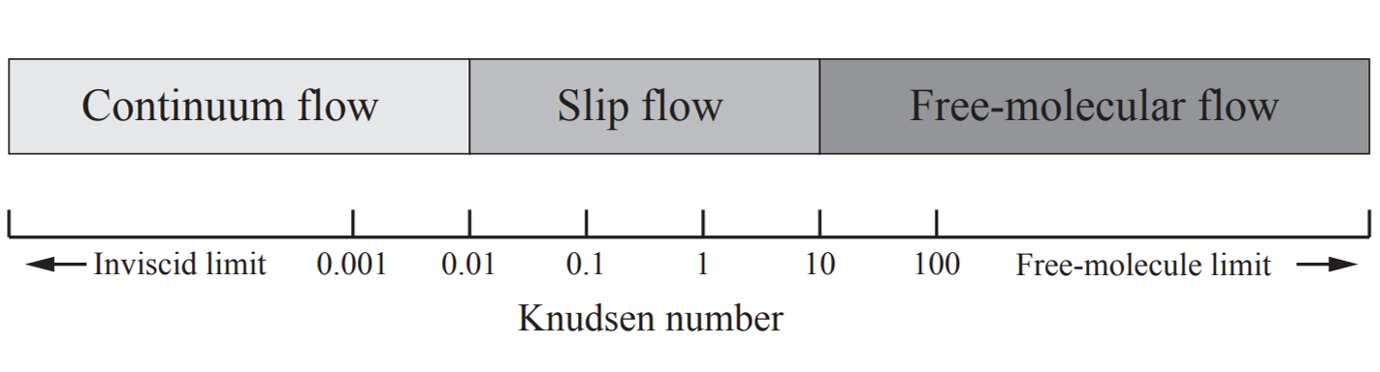
\includegraphics[width=0.7\textwidth]{../Images/2. Background/regimes.png}
    \caption{Flow regime with varying Knudsen number \cite{aerothermonotes}.}
    \label{fig:regimes}
\end{figure}
\begin{itemize}
    \item For Knudsen numbers below 10\textsuperscript{-2}, the flow can be classified as continuum. This kind of flow is characterised with a very significant number of intermolecular collision \cite{aerothermonotes, chambrerarefied}, and is commonly observed in everyday conditions, such as the flow around the wing of an aircraft or the flow of water in a pipe. It can be mathematically modelled through the Navier-Stokes equations.
    \item For Knudsen numbers between 10\textsuperscript{-2} and 10\textsuperscript{1}, flow can be classified as slip. In this condition the number of collisions between molecules is low, but not negligible \cite{chambrerarefied}. This leads to notable phenomena such as the boundary temperature jump, where the flow temperature at the wall differs from the surface wall temperature \cite{slipjump}. Moreover, a boundary slip velocity condition arises, which negates the the no-slip condition observed in ordinary flows \cite{slipjump}. These phenomena are schematically represented in \autoref{fig:slipjump}. The modelling of this regime depends on $Kn$. For conditions which approach the continuum flow, this regime can be modeled by incorporating correction factors into the Navier stokes equations \cite{slipjump} (in order to account for the aforementioned phenomena). Alternatively, it can be described through the Burnett and super Burnett equations \cite{burnett}.
    \item For Knudsen numbers above 10\textsuperscript{1}, the flow is classified as free molecular flow. In this regime, intermolecular collisions are so rare that the notion of an ordered flow of molecules ceases to exist \cite{aerothermonotes, chambrerarefied}, and is replaced by a statistical description, in the form of the Boltzmann equation, which can be seen in 
\end{itemize}
\begin{figure}[ht]
    \centering
    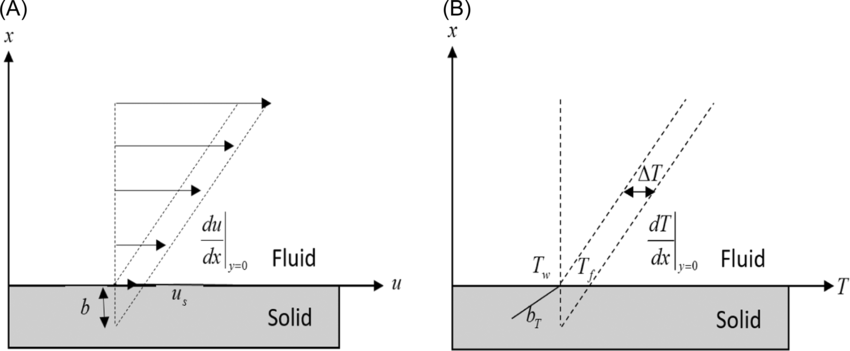
\includegraphics[width=0.7\textwidth]{../Images/2. Background/slipjump.png}
    \caption{Schematic diagram of velocity slip (A) and temperature jump (B)  \cite{slipjump}.}
    \label{fig:slipjump}
\end{figure}

It is important to note that while a flow may be globally continuous, certain local regions may exhibit signs of rarefied flow. An illustrative example of this phenomenon is the re-entry path of the space shuttle. While the global Knudsen number, calculated based on the length of the vehicle, may fall within the continuum regime, the Knudsen number associated with the flow around one of the rivets on its wing could differ significantly, potentially resulting in a different flow regime altogether.

ADD HATHORAERO2

\subsection{Rarefied flow modelling}
As mentioned previously, Navier-Stokes equations cease to be valid in the rarefied flow regime. Different methods thus need to be employed for its analytical description.

Free molecular flow is modelled through the Boltzmann equation, presented in \autoref{eq:boltzmann} in its multi species form. In \autoref{eq:boltzmann}, $\mathbf{F}(r, t)$ is the force field acting on the fluid particles

\begin{equation}
    \frac{\partial f_i}{\partial t}+\frac{\mathbf{p}_i}{m_i} \cdot \nabla f_i+\mathbf{F} \cdot \frac{\partial f_i}{\partial \mathbf{p}_i}=\left(\frac{\partial f_i}{\partial t}\right)_{\text {coll }}
    \label{eq:boltzmann}
\end{equation}
